\chapter{Die schwerwiegende moralische Entscheidung}

Am 27. September 1983 stießen die Programmierer, die die Usenet-Newsgroup net.unix-wizards lasen, auf eine ungewöhnliche Nachricht. Das Posting war in den frühen Morgenstunden, genauer gesagt um 0:30, abgeschickt worden und stammte von \url{rms@mit-oz}. Die Betreffzeile war kurz, aber aufmerksamkeitserregend: "`Neue UNIX-Implementation"'. Jedoch gab es statt einer neuen Version von Unix im ersten Abschnitt einen Aufruf, zu den Waffen zu greifen:

\begin{quote}
Ab diesem Thanksgiving\footnote{Thanksgiving wird am vierten Donnerstag im November gefeiert.} werde ich ein vollständiges unixkompatibles Softwaresystem namens GNU (für Gnu's Not Unix) schreiben und jedem gratis geben, der es gebrauchen kann. Beiträge in Form von Zeit, Geld, Programmen und Ausrüstung werden dringend benötigt.\footcite[Vgl.][]{rmsgnuan}\index{GNU Announcement}
\end{quote}

Für einen erfahrenen Unix-Entwickler stellte diese Nachricht eine Mischung aus Idealismus und Übermut dar. Nicht nur versprach der Autor, das gesamte, bereits ausgereifte Unix-Betriebssystem von Grund auf nachzubauen, er schlug auch noch vor, es stellenweise zu verbessern. Das neue GNU-System, so der Autor, sollte alle üblichen Komponenten beinhalten – einen Texteditor, eine Shell\comment{zum Ausführen Unix-kompatibler Anwendungen}, einen Compiler und "`ein paar andere Dinge"'.\footcite{rmsgnuan} Es sollte auch viele verlockende Funktionen enthalten, die andere Unix-Systeme noch nicht boten: eine graphische Benutzerschnittstelle auf der Basis von Lisp, ein absturzsicheres Dateisystem und Netzwerksoftware auf der Basis von Chaosnet, dem MIT-internen Netzwerksystem.

"`GNU wird in der Lage sein, alle Unix-Programme auszuführen, aber nicht identisch mit Unix sein"', schrieb der Autor. "`Wir werden alle Verbesserungen machen, die praktisch sind, basierend auf unserer Erfahrung mit anderen Betriebssystemen."'

Um den skeptischen Fragen der Leser vorzugreifen, gibt der Autor nach seiner Betriebssystemskizze einen kurzen biographischen Überblick, überschrieben mit "`Wer bin ich?"':

\begin{quote}
Ich bin Richard Stallman, Erfinder des oft imitierten, originalen EMACS-Editors, gegenwärtig [tätig] am Artificial Intelligence Lab des MIT. Ich habe ausgiebig an Compilern, Editoren, Debuggern, Befehlsinterpretern, dem Incompatible Timesharing System und dem Betriebssystem der Lisp-Maschine gearbeitet. Ich habe auf dem Gebiet des terminalunabhängigen Displaysupports in ITS Pionierarbeit geleistet. Des weiteren habe ich ein absturzsicheres Dateisystem und zwei Fenstersysteme für die Lisp-Maschine implementiert.\footcite{rmsgnuan}
\end{quote}

Wie es das Schicksal wollte, konnte das von Stallman gesetzte Startdatum für das ambitionierte GNU Project nicht gehalten werden. Im Januar 1984 konnte Stallman sein Versprechen einlösen und sich voll der Unix-Softwareentwicklung widmen. Für einen Softwarearchitekten, der mit ITS großgeworden ist, war das als würde ein Architekt von maurischen Palästen plötzlich Einkaufszentren in der Vorstadt planen. Ungeachtet dessen hatte das Bauen eines unixoiden Betriebssystems seine versteckten Vorteile. ITS war mächtig, aber es hatte auch eine Achillesferse: die MIT-Hacker hatten es speziell für die leistungsfähige PDP-10 von DEC geschrieben. Als sich die Administratoren\comment{administrators} des AI~Labs Anfang der 80er entschieden, die PDP-10 aus dem Verkehr zu ziehen, wurde das Betriebssystem, das die Hacker einst mit einer pulsierenden Stadt verglichen, unmittelbar zu einer Geisterstadt. Unix andererseits war mit Portabilität im Hinterkopf entworfen, was es für solche Gefahren unempfänglich machte. Das ursprünglich von jungen Wissenschaftlern an AT\&Ts Bell Labs entwickelte System war nicht auf dem Radar der Firmenleitung aufgetaucht und fand ein glückliches Zuhause in der Welt der akademischen Computersysteme, die immer knapp bei Kasse war. Den Unix-Entwicklern standen geringere Ressourcen als ihren MIT-Kollegen zur Verfügung; sie hatten die Software so angepasst, dass sie auf anderen Systemen läuft, hauptsächlich der 16-bittigen PDP-11 – ein Rechner, der von den meisten AI-Lab-Hackern nur als für kleine Aufgaben geeignet angesehen wurde – aber später auch auf 32-Bit-Mainframes wie der VAX 11/780. Bis zum Jahr 1983 begannen einige Unternehmen, insbesondere Sun Microsystems, damit, eine leistungsfähigere Klasse von Desktopcomputern zu entwickeln, "`Workstations"', um das sich zunehmend verbreitende  Betriebssystem auf Rechnern einzusetzen, die in Sachen Leistung der viel älteren PDP-10 entsprachen.

% TODO: impliziert, Original-Unix wäre in C geschrieben worden
% http://oreilly.com/catalog/opensources/book/kirkmck.html
Um die Portabilität zu erleichtern, haben die Unix-Entwickler eine weitere Abstraktionsschicht zwischen die Software und die Hardware gelegt. Statt es in einer speziellen Maschinensprache zu schreiben – wie die AI-Lab-Hacker mit ITS auf der PDP-10 – haben die Unix-Entwickler es in einer Hochsprache, getauft auf den Namen C, geschrieben. Sie konzentrierten sich mehr auf die ineinandergreifenden Schnittstellen und die Spezifikationen, die die vielen Subkomponenten zusammenhalten, als auf die Komponenten selbst, und schufen ein System, das man schnell auf andere Systeme anpassen konnte. Wenn einem Nutzer eine bestimmte Komponente nicht gefiel, konnte er mit der Schnittstellenspezifikation eine einzelne Subkomponente herausnehmen und sie bereinigen oder mit etwas besserem ersetzen. Einfach gesagt, förderte der Unix-Ansatz Flexibilität und Wirtschaftlichkeit, daher seine schnelle Verbreitung.\footcitet[Vgl.][S. 38: Marshall Kirk McKusick, \textit{Twenty Years of Berkeley Unix}]{opensrc} 

Stallmans Entscheidung, die Entwicklung des GNU-Systems zu starten, wurde durch das Ende des ITS-Systems ausgelöst, das die AI-Lab-Hacker so lange gehegt hatten. Der Niedergang von ITS und der AI-Lab-Hackergemeinde, die es am Leben gehalten hatte, mit ihm, war ein traumatischer Schlag für Stallman. Wenn ihn der Vorfall mit dem Xerox-Laserdrucker gelehrt hatte, die Ungerechtigkeit proprietärer Software zu erkennen, zwang ihn das Sterben seiner Gemeinde, sich zu entscheiden, ob er vor der proprietären Software kapituliert oder sich ihr entgegensetzt.

Wie der Code, aus dem es bestand, lagen die Wurzeln von ITSs Niedergang weit in der Vergangenheit. Bis 1980 arbeiteten die meisten Hacker im Lab an der Entwicklung der Lisp-Maschine und seines Betriebssystems.

Lisp, erfunden von einem Pionier im Bereich der Künstlichen Intelligenz und KI-Forscher am MIT während der späten 50er, John McCarthy\index{McCarthy, John}, ist eine elegante Sprache, die sich gut eignet, komplexe Programme zu schreiben, die mit unregelmäßigen Datenstrukturen operieren. Der Name der Sprache ist die Kurzform für "`LISt Processing"'. Nachdem McCarthy zum Stanford Artificial Intelligence Laboratory gewechselt war, entwickelten MIT-Hacker einen Lisp-Dialekt namens "`MACLISP"'. Das "`MAC"' kommt von dem Project MAC, dem DARPA-finanzierten Forschungsprojekt, aus dem das AI~Lab und das Laboratory for Computer Science hervorgingen. Angeführt vom Urhacker Richard Greenblatt\index{Greenblatt, Richard|(} entwickelten die AI-Lab-Hacker Ende der 70er einen Computer, der darauf spezialisiert war, Lisp-Programme effizient und bequem auszuführen, die Lisp-Maschine, und dann ein komplettes Lisp-basiertes Betriebssystem für sie.

%Abschnitt geändert
1979\comment{OT: 1980} hatten zwei rivalisierende Hackergruppen Firmen gegründet, die Lisp-Maschinen herstellen und verkaufen. Greenblatt\index{Greenblatt, Richard|)} gründete Lisp Machines Incorporated. Er wollte Einflüsse von Kapitalgebern vermeiden und eine "`Hacker-Firma"' haben. Die meisten Hacker schlossen sich Symbolics an, einem normalen Startup. 1982 hörten sie völlig auf, am MIT zu arbeiten.

Mit den paar Hackern, die noch übrig waren, sich um den Laden zu kümmern, dauerte es länger, die Programme und Rechner zu reparieren – oder sie wurden gleich gar nicht repariert. Was noch schlimmer war, so Stallman, war der "`demographische Wandel"' im Lab. Die Hacker, die einst eine lautstarke Minderheit im AI~Lab bildeten, waren fast alle weg, aber "`die Professoren und Studenten, die die [PDP-10] nicht wirklich mochten, waren immer noch so zahlreich wie vorher."'\footcite{rmskth}

1982 erhielt das AI~Lab Ersatz für seinen Zentralcomputer, die PDP-10, der über 12 Jahre alt war. DECs aktuelles Modell, das Decsystem 20, war kompatibel mit den Anwenderprogrammen, aber eine radikale Anpassung oder "`Portierung"' wäre nötig gewesen, hätten die Hacker das alte Betriebssystem ITS weiterverwenden wollen. Aus Angst darüber, dass das Lab seine kritische Masse an internen Programmiertalenten verloren hatte, drängte das AI-Lab-Personal zu Twenex, einem kommerziellen Betriebssystem von DEC. Die Hacker wurden überstimmt und mussten sich beugen.

\begin{figure}[ht] \centering
  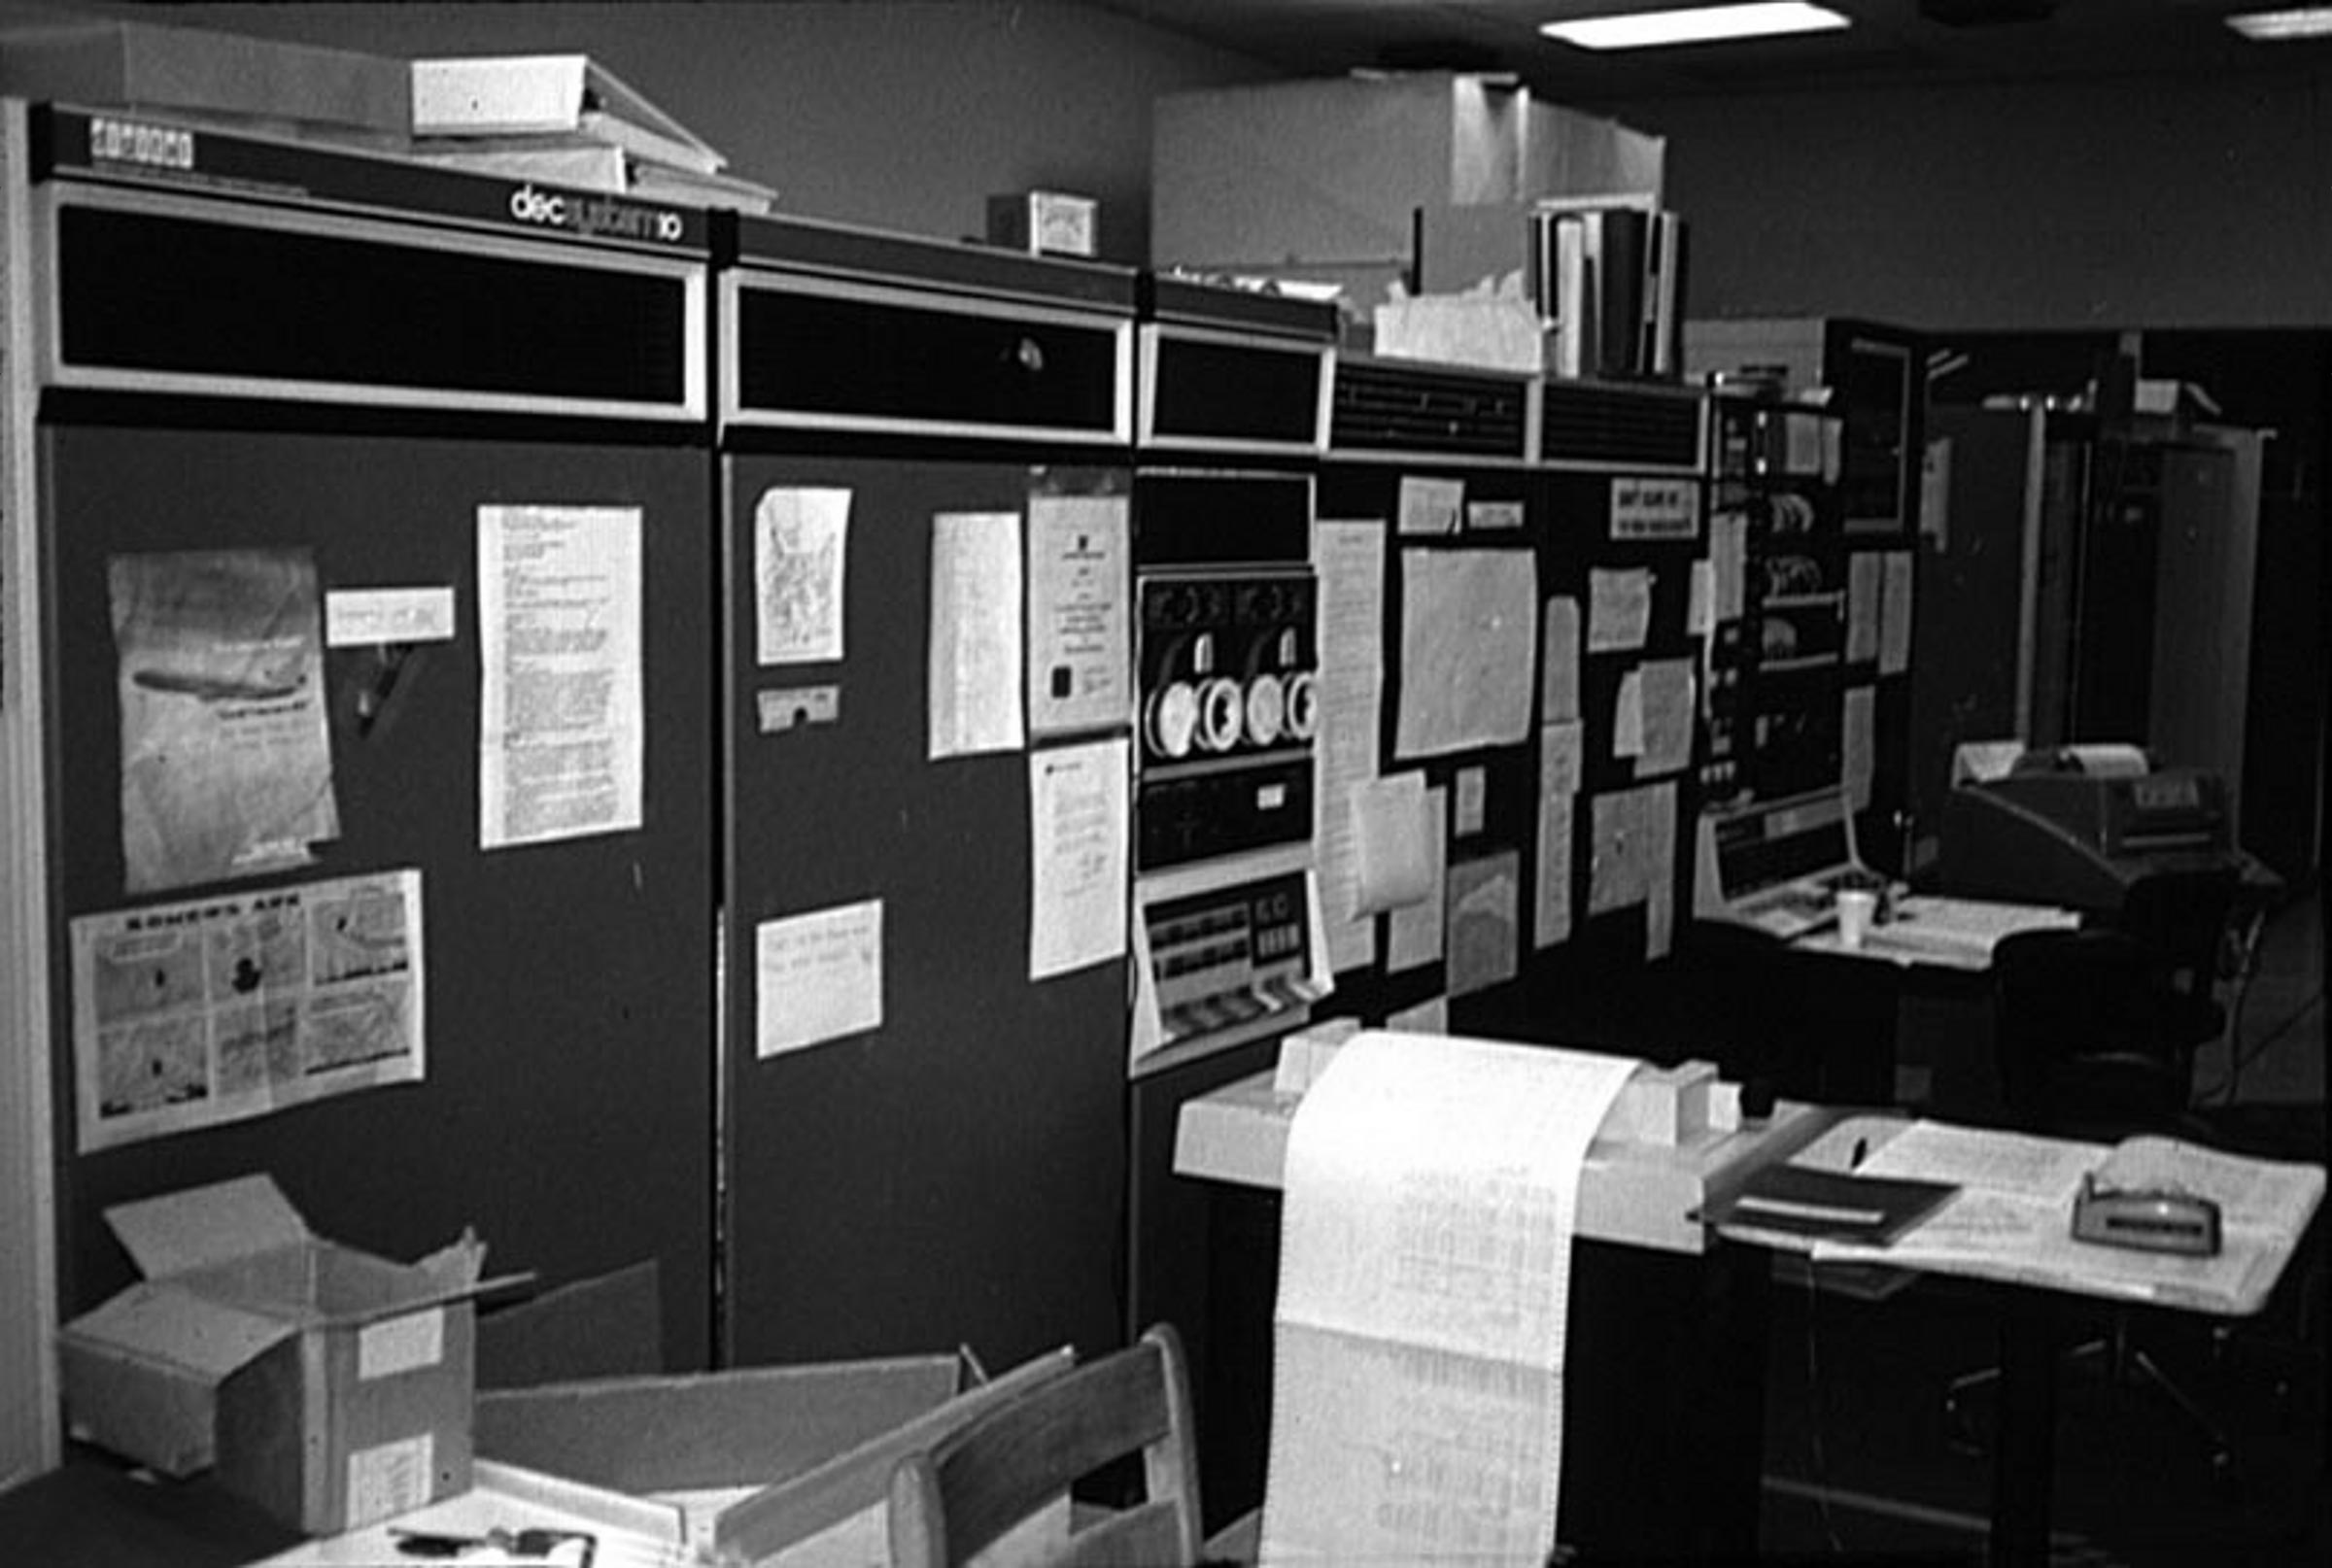
\includegraphics[width=0.8\textwidth]{KL10_1979}
  \caption{\small PDP-10-Rechenanlage mit Zentraleinheit KL-10 (ähnlich der im AI Lab), Stanford Artificial Intelligence Laboratory, 1979.}
\end{figure}

"`Ohne Hacker, die das System warten, haben die [Dozenten] gesagt, \glq Das gibt ein Desaster; wir brauchen kommerzielle Software.\grq\,"', erinnert sich Stallman einige Jahre später. "`Sie haben gesagt \glq Wir können von der Firma erwarten, dass sie es warten.\grq{} Das hat sich als völlig falsch erwiesen, aber sie haben es so gesagt.\comment{but that's what they did}"'\footcite{rmskth}

Zuerst haben die Hacker das Twenenx-System\index{Twenex|(} nur als weiteres Symbol des Autoritarismus angesehen, das danach schreit, umgestürzt zu werden. Der Systemname selbst war schon ein Protest. Das von DEC offiziell so genannte, und nach seinem Vorgänger TOPS-10 benannte, proprietäre Betriebssystem TOPS-20 wurde für die PDP-10 vertrieben. Aber TOPS-20 basierte nicht auf TOPS-10. Es war vom Tenex-System\index{Tenex} abgeleitet, das Bolt Beranek Newman für die PDP-10 entwickelt hatte.\footnote{Mehrere Quellen: Interview mit Richard Stallman, E-Mail von Gerald Sussman und \cite[][Glossary: "`TWENEX"']{jargonf}.} Stallman, der den Begriff "`Twenex"' geprägt hat, sagt, er ist darauf gekommen, weil er den Namen TOPS-20 vermeiden wollte. "`Das System war weit davon entfernt, top zu sein, und deshalb wollte ich es um keinen Preis so nennen"', erinnert sich Stallman. "`Also habe ich mich entschieden, ein \glq w\grq{} in den Namen Tenex einzufügen und es Twenex zu nennen."'

%Zitate aus zwei verschiedenen Szenen aus dem Film von 1939
%Buch: "Ich bin der große und schreckliche Oz."
%"Beachtet nicht weiter den Mann hinter dem Vorhang." -> nicht im Buch
Der Rechner, auf dem das Betriebssystem Twenex/TOPS-20 lief, hatte seinen eigenen spöttischen Spitznamen: Oz. Der Hackerlegende zufolge erhielt der Rechner seinen Namen, weil er eine kleinere PDP-11 benötigte, um das Terminal zu betreiben. Ein Hacker, der den KL-10/PDP-11-Aufbau zum ersten Mal sah, verglich ihn mit der bombastischen filmischen Vorstellung des Zauberers von Oz. "`Ich bin Oz, der große und mächtige"', tönte der Hacker. "`Beachtet nicht weiter die PDP-11 hinter der Konsole."'\footcite[Vgl.][]{fig1}

Auch wenn die Hacker zuerst gelacht haben, wenn sie die KL-10 das erste Mal gesehen haben, sollte ihr Gelächter schnell verstummen, wenn sie es mit Twenex zu tun bekamen. Nicht nur rühmte sich Twenex\index{Twenex|)} seiner integrierten Sicherheitsvorkehrungen, die Systemingenieure hatten die Werkzeuge und Anwendungen auch mit Sicherheitsaspekten im Hinterkopf entworfen. Was einst ein Katz-und-Maus-Spiel wegen Passwörtern auf dem Sicherheitssystem des Laboratory for Computer Science war, war zu einem absoluten Kampf um die Systemverwaltung geworden. Die Systemadministratoren argumentierten, dass das Oz-System ohne Sicherheitsvorkehrungen anfälliger für versehentliche Abstürze wäre. Die Hacker argumentierten, dass das besser durch Überarbeitung des Quellcodes vermieden werden könne. Unglücklicherweise war die Anzahl der Hacker mit der Zeit für und der Neigung zu dieser Art Überarbeitung soweit geschwunden, dass sich die Ansichten der Administratoren durchsetzten.

Anfangs war es Praxis, dass jedes Mitglied des AI Labs das "`Wheel"'-Privileg\index{Wheel}\footnote{Der Begriff taucht das erste mal in TENEX auf und ist die Kurzform für "`big wheel"'. \cite[Vgl.][Glossary: "`wheel"']{jargonf}.} hatte, um die Sicherheitsbeschränkungen zu umgehen. Aber jeder, der das "`Wheel"'-Privileg hatte, konnte es jedem anderen streichen, und dann hatte derjenige keine Möglichkeit mehr, es wiederherzustellen. Diese Situation führte dazu, dass eine kleine Gruppe Hacker versucht war, mit dem Entfernen der "`Wheel"'-Privilegien der anderen die völlige Kontrolle an sich zu reißen.

Durch das Schnorren von Passwörtern und Debuggen konnte Stallman die Vorhaben vereiteln. Nach dem zweiten gescheitertem \textit{Coup d'État} gab Stallman eine Warnung an das AI-Lab-Personal heraus.\footcite[Vgl.][]{rmskth}

"`Es hat wieder einen Versuch gegeben, die Macht zu ergreifen"', schrieb Stallman. "`Fürs Erste sind die aristokratischen Truppen geschlagen."' Um seine Identität zu verschleiern, unterschrieb Stallman die Nachricht mit "`Radio Free OZ"'.

Die Tarnung war bestenfalls dürftig. 1982 war Stallmans Abneigung gegen Passwörter und Geheimhaltung so bekannt geworden, dass Leute außerhalb des AI Laboratory sein Benutzerkonto von überall aus dem ARPAnet nutzten – dem mit Forschungsgeldern finanzierten Computernetzwerk, das dem Internet als Grundlage dienen sollte. Einer dieser "`Touristen"' während dem Anfang der 80er war Don Hopkins\index{Hopkins, Don|(}, ein kalifornischer Programmierer, der über Gerüchte erfahren hatte, dass man sich als Außenstehender einfach mit dem Benutzernamen RMS und demselben Passwort an MITs gepriesenem ITS-System anmelden konnte.

"`Ich bin dem MIT auf ewig dankbar, dass sie mich und viele andere ihre Computer umsonst haben nutzen lassen"', sagt Hopkins\index{Hopkins, Don|)}. "`Es hat einer Menge Leute viel bedeutet"'.

Der sogenannte "`Tourismus"', der von der MIT-Leitung in den ITS-Jahren toleriert wurde,\footcite{mittour} blieb auf der Strecke, als Oz die Hauptverbindung des AI Labs ins ARPAnet wurde. Zuerst hielt Stallman an der Tradition fest, seinen Benutzernamen als Passwort zu verwenden, damit Nutzer von außerhalb Zugang über sein Konto erlangen konnten. Mit der Zeit veranlasste die Instabilität von Oz die Administratoren jedoch dazu, Außenstehende zu blockieren, die versehentlich oder mit Absicht das System abschießen könnten. Als diese Administratoren schließlich von Stallman verlangten, sein Passwort nicht mehr zu veröffentlichen, berief sich Stallman auf seine persönliche Ethik und hörte ganz auf, das System zu benutzen.\footcite[Vgl.][]{rmskth}

"`Seitdem Passwörter im MIT AI~Lab aufgetaucht sind, habe ich [mich entschieden], meiner Überzeugung zu folgen, dass es keine Passwörter geben sollte"', sagt Stallman später. "`Weil ich nicht glaube, dass es wirklich erstrebenswert ist, Sicherheitsmaßnahmen auf einem Computer zu haben, sollte ich nicht gewillt sein, das Aufrechterhalten eines Sicherheitsregimes zu unterstützten."'\footcite{rmskth}

Stallmans Weigerung, sich dem großen und mächtigen Oz zu beugen, symbolisierte die wachsende Spannung zwischen den Hackern und der AI-Lab-Leitung Anfang der 80er. Die Spannung war kein Vergleich zu den Konflikten, die sich in der Hackergemeinschaft selbst abspielten. Als das Decsystem 20 ankam, war die Gemeinschaft in zwei Lager gespalten – LMI und Symbolics.

Symbolics mit seinem Fremdkapital heuerte verschiedene AI-Lab-Hacker an. Einige von ihnen setzte man außerhalb des AI~Labs zur Verbesserung von Betriebssystemteilen der Lisp-Maschine ein. Ende 1980 arbeiteten 14 Mitglieder des AI~Labs in Teilzeit als Berater an der Entwicklung einer eigenen Version der Lisp-Maschine für die Firma. Die wenigen übrigen, außer Stallman, arbeiteten für LMI.\footcite[Vgl.][S.\,423]{hackers} Stallman, der das ungezwungene Leben am AI~Lab bevorzugte und keine Partei ergreifen wollte, entschied sich, keinem der beiden Unternehmen beizutreten.

Zuerst verbrachten die anderen Hacker weiterhin Zeit am MIT und leisteten ihre Beiträge zum Betriebssystem der MIT-Lisp-Maschine. LMI und Symbolics hatten beide den Code vom MIT lizenziert. Die Lizenz erforderte es, dass sie ihre Änderungen an das MIT zurückgeben, aber sie mussten es dem MIT nicht erlauben, diese Änderungen weiterzuverbreiten. Jedoch hielten sie sich bis 1981 an ein Gentlemen's Agreement, dass es zuließ, und so konnten alle Systemverbesserungen in die MIT-Version eingehen und mit allen Nutzern von Lisp-Maschinen geteilt werden. Diese Situation erlaubte es den am MIT Verbliebenen, neutral zu bleiben.

Am 16. März 1982, erinnert sich Stallman, weil es an seinem Geburtstag war, kündigte Symbolics das Gentlemen's Agreement auf. Das Motiv war ein Angriff auf LMI. LMI hatte weniger Hacker und allgemein weniger Personal, also dachte der Symbolics-Vorstand, dass LMI den größten Vorteil aus dem Teilen der Verbesserungen zog. Mit der Aufkündigung des Systemcodeaustausches hofften sie, LMI auszulöschen. Sie entschieden sich, die Lizenz exakt durchzusetzen. Statt ihre Verbesserungen in die MIT-Version des Systems einzuarbeiten, welches LMI nutzen konnte, stellten sie dem MIT eine Kopie der Symbolics-Version des Systems zur Verfügung\comment{, die die Nutzer am MIT verwenden konnten}. Jeder, der das System benutzte, würde nur für Symbolics Testarbeit leisten, und wenn er Verbesserungen machte, wären sie höchstwahrscheinlich auch nur für Symbolics von Nutzen.

Als Verantwortlicher (in den ersten Monaten mit Hilfe Greenblatts\index{Greenblatt, Richard}) für die Wartung der Lisp-Maschinen im Labor war Stallman empört. Die Symbolics-Hacker hatten den Code des Systems mit hunderten halbfertigen Änderungen zurückgelassen, die Fehler verursachten. Er sah diese Ankündigung als "`Ultimatum"' an und revanchierte sich, indem er Symbolics' Richtfunkverbindung\comment{microwave communications link} zum AI~Lab kappte. Er schwor sich, nie wieder an einer Symbolics-Maschine zu arbeiten und das MIT-System weiterzuentwickeln, um LMI gegen Symbolics zu verteidigen. "`So wie ich es gesehen habe, war das AI~Lab neutrales Territorium wie Belgien im Zweiten Weltkrieg"', sagt Stallman. "`Wenn Deutschland in Belgien einfällt, dann erklärt Belgien Deutschland den Krieg und verbündet sich mit Britannien und Frankreich."'

Als der Symbolics-Vorstand merkte, dass ihre neuesten Funktionen immer noch auf den Lisp-Maschinen des MIT auftauchten und somit auch in den Lisp-Maschinen von LMI, waren sie nicht erfreut. Stallman wusste, was das Urheberrecht erfordert, und schrieb die Funktionen komplett neu. Er nutzte die Möglichkeit aus, sich den Quellcode anzuschauen, den Symbolics dem MIT zur Verfügung stellte, so dass er die Probleme und ihre Lösungen verstand, und achtete dann darauf, seine Änderungen auf eine ganz andere Weise zu schreiben. Der Symbolics-Vorstand wollte das nicht glauben. Sie installierten ein "`Spionage"'-Programm auf Stallmans Terminal, das nach Beweisen gegen ihn suchen sollte. Als sie ihr Anliegen dann der MIT-Leitung vorbrachten, etwa Anfang 1983, hatten sie wenig Beweise vorzuweisen: ein Dutzend Stellen im Quellcode, an denen beide Versionen geändert wurden und ähnlich aussahen.

Als die Leiter des AI~Labs Stallman die mutmaßlichen Beweise von Symbolics zeigten, entkräftete er sie, indem er bewies, dass die Ähnlichkeiten in Wirklichkeit Relikte aus der Zeit vor dem Fork waren. Und er drehte ihre Logik um: wenn Symbolics bei den tausenden Zeilen, die er geschrieben hatte, mit keinen besseren Beweisen aufwarten konnte, wies das nach, dass seine sorgfältigen Anstrengungen, Plagiate zu vermeiden, wirksam waren. Das AI~Lab hieß Stallmans Arbeit gut, und er führte sie bis Ende 1983 fort.\footnote{Im Buch \citefield{title}{brainm} behauptet der Autor \citeauthor{brainm} fälschlich, dass das AI~Lab ihn angewiesen hat, sich aus dem Lisp-Maschinen-Projekt herauszuhalten.}

Dennoch änderte Stallman seine Taktik. "`Nur um ultrasicher zu sein, habe ich deren Quellcode nicht mehr gelesen. Ich habe nur die Dokumentation [als Grundlage] verwendet und den Code damit geschrieben."'  Die größten neuen Funktionen entwarf er selbst, ohne auf die Veröffentlichung der Dokumentation von Symbolics zu warten. Wenn die Dokumentation dann erschien, machte er sie mit der Symbolics-Schnittstelle für die Funktion kompatibel. Danach las er Symbolics' Quellcodeänderungen, um auch kleinere Fehler zu finden, die sie behoben hatten, und behob sie selbst auf eine andere Art.

Die Erfahrung stärkte Stallmans Entschlossenheit. Stallman heuerte außerdem Mitglieder des AI~Labs an, die das MIT-System weiter nutzen sollten, damit der Fluss an Fehlerreports für seine Ersatzfunktionen nicht abbricht. Das MIT gewährte LMI weiterhin direkten Zugriff auf die Änderungen. "`Ich wollte Symbolics bestrafen, auch wenn es das letzte sein sollte, was ich tue"', sagt Stallman. Solche Äußerungen sind aufschlussreich. Sie bringen nicht nur Licht an Stallmans nichtpazifistische Natur, sie spiegeln auch die intensiven Gefühle wider, die der Konflikt bei ihm ausgelöst hat.

Das Ausmaß der Verzweiflung war stark dem geschuldet, was Stallman als "`Zerstörung"' seines "`Zuhauses"' betrachtete – dem Niedergang der eng verbundenen Hackersubkultur. In einer der letzten Interview-E-Mails sollte sich Stallman mit der historischen Figur Ishi vergleichen, dem letzten überlebenden Mitglied der Yahi, einem Indianerstamm im Pazifischen Nordwesten, der in den Indianerkriegen in den 1860ern und 1870ern ausgerottet wurde. Die Analogie stellt Stallmans Überleben in ein episches, fast mythisches Licht.\footnote{Steven Levy hatte in \citefield{shorttitle}{hackers} diese Zeit im Sinn, als er Stallman als den "`letzten echten Hacker"' bezeichnete, aber die beabsichtigte Bedeutung ist anders, als man vielleicht denken mag. Levy benutzte den Begriff "`echte Hacker"' zur Unterscheidung der MIT-Hackergemeinde von den zwei anderen Hackergemeinden im Buch, die später beschrieben werden und die er anders bezeichnet. Als sich seine Gemeinde aufgelöst hatte und nur Stallman übrig war, wurde er damit zum letzten "`echten Hacker"'. Levy meint nicht, dass niemand sonst ein wahrhaftiger Hacker ist, aber man scheint es meist so zu interpretieren\comment{, besonders die Leute, die sich nicht die Erläuterungen in Levys Buch durchlesen}. Stallman selbst hat sich nie mit diesen Worten beschrieben.} Die Hacker, die für Symbolics arbeiteten, sahen das anders. Statt Symbolics als zerstörerische Kraft anzusehen, sahen es viele Kollegen Stallmans als späten Versuch, sich Geltung zu verschaffen. Mit der Kommerzialisierung der Lisp-Maschine hatte die Firma die Hackerprinzipien des ingenieurgetriebenen Softwaredesigns aus dem Elfenbeinturm des AI~Labs in den Unternehmensmarkt gedrängt, auf dem die Designprinzipien der Manager vorherrschten. Statt Stallman als einen Verweigerer zu sehen, sahen viele in ihm einen Repräsentanten einer veralteten Praxis.

Auch persönliche Feindseligkeiten spielten eine Rolle. Selbst bevor Symbolics die meisten AI-Lab-Hacker abgeworben hatte, sagt Stallman, hätten ihn viele der Hacker, die später zu Symbolics gehen sollten, gemieden. "`Man hat mich nicht mehr nach Chinatown eingeladen"', entsinnt sich Stallman. "`Der von Greenblatt gestartete Brauch war, dass wenn man auswärts zu Abend isst, man herumgeht und die anderen im Lab fragt oder eine Nachricht schickt, ob sie auch mitkommen wollen. Irgendwann um 1980-1981 hat es aufgehört, dass ich gefragt wurde. Sie haben mich nicht nur nicht gefragt, aber jemand hat mir später gestanden, dass er unter Druck gesetzt worden ist, mich zu belügen und das Essengehen ohne mich geheimzuhalten."'

Obwohl sich Stallman von dieser engstirnigen Form der Ausschließung verletzt fühlte, konnte er nichts dagegen tun. Das Ultimatum von Symbolics änderte den Sachverhalt von einer persönlichen Ablehnung zu einer größeren Ungerechtigkeit. Als Symbolics seine Quellcodeänderungen von der Weiterverbreitung ausnahm, um seinen Rivalen zu schlagen, entschied sich Stallman, ihre Pläne zu durchkreuzen. Indem er mit seinen Aufgaben am MIT durchhält und ein Gegenstück zu jeder neuen Softwarefunktion und jedem Fix schreibt, wollte er den Nutzern des MIT-Systems, einschließlich den LMI-Kunden, dieselbe Funktionalität geben, die die Symbolics-Nutzer hatten.

Außerdem würde es Stallmans Status als Legende in der Hackergemeinde sichern sollen. Schon damals war er berühmt für seine Arbeit an Emacs, und seine Fähigkeit, mit der Arbeitsleistung eines ganzen Teams von Symbolics-Programmierern gleichzuziehen – einem Team, das selbst mehr als nur ein paar legendäre Hacker umfasste – steht heute immer noch als eine der größten Leistungen des Informationszeitalters, oder jedes Zeitalters. Steven Levy bezeichnete es als einen "`Meister-Hack"' und Stallman selbst als einen "`virtuellen John Henry des Computercodes"'.\footnote{John Henry ist ein US-amerikanischer Folkloreheld, der in einem Wettkampf bei Gleisverlegearbeiten gegen einen Dampfhammer gewonnen haben soll.} Er merkt an, dass selbst seine bei Symbolics angestellten Rivalen keine Wahl hatten, als ihrem idealistischen alten Kameraden widerwillig Respekt zu zollen. Levy zitiert Bill Gosper\index{Gosper, Ralph William \glq Bill\grq}, einen Hacker, der in ihrem Büro in Palo Alto für Symbolics arbeitete, wie er sein Erstaunen über Stallmans Programmierleistungen in dieser Phase ausdrückt:

\begin{quote}
Ich sah etwas, was Stallman geschrieben hat, und ich würde es vielleicht für schlecht befinden (eher nicht, aber man könnte mich überzeugen, dass es schlecht war), aber dann würde ich immer noch sagen, "`Ja, Moment mal – Stallman hat da drüben niemanden, mit dem er die ganze Nacht diskutieren kann. Er arbeitet allein! Es ist unglaublich, dass jemand das alles allein machen kann!"'\footcite[Vgl.][S.\,426]{hackers}
\end{quote}

%machine room - 
Für Stallman rufen die Monate, die er damit verbracht hat, mit Symbolics aufzuholen, eine Mischung aus Stolz und tiefer Traurigkeit hervor. Stallman, ausgemachter Linker, dessen Vater im Zweiten Weltkrieg gedient hatte, ist kein Pazifist. In vielerlei Hinsicht war der Symbolics-Krieg der Initiationsritus, auf den Stallman seit Beginn seiner Anstellung am AI~Lab ein Jahrzehnt zuvor hingeschlittert ist. Und gleichzeitig fiel er mit der traumatischen Zerstörung der Hackerkultur am AI~Lab zusammen, die Stallman seit seiner Jugend aufgezogen hatte. Eines Tages, als er eine Programmierpause machte, hatte Stallman ein traumatisches Erlebnis beim Durchgehen durch den Rechnerraum des Labs. Dort sah Stallman das klobige, ungenutzte Gehäuse einer PDP-10. Bestürzt über die erloschenen Lämpchen, die einst eifrig blinkten und den internen Zustand von Systemprogrammen anzeigten, war der emotionale Einfluss auf Stallman ähnlich dem, ein geliebtes Familienmitglied aufgebahrt zu sehen.

"`Ich habe direkt dort im Rechnerraum angefangen, zu weinen"', sagt er. "`Die Maschine dort zu sehen, tot, ohne jemanden, der sie reparieren kann, hat mir klargemacht, wie völlig zerstört meine Gemeinde gewesen ist."'

Stallman sollte wenig Zeit zum Trauern bleiben. Die Lisp-Maschine war, trotz all dem Aufruhr um sie und all der Arbeit, die in ihre Entwicklung geflossen ist, nur ein Nebenkriegsschauplatz in der größeren Schlacht auf dem technologischen Markt. Die unermüdliche Geschwindigkeit der Computerminiaturisierung brachte immer neue, leistungsfähigere Mikroprozessoren hervor\comment{, die die Hardware- und Softwarefähigkeiten der Maschine verschlingen würde wie eine moderne Metropole ein vorzeitliches Wüstendorf XXX would soon incorporate the machine's hardware and software capabilities like a modern metropolis swallowing up an ancient desert village}.

Mit dieser Welle kamen hunderte, ja tausende, proprietäre Softwareprogramme, jedes davon geschützt durch ein Geflecht an Endnutzer-Lizenzvereinbarungen und Geheimhaltungsverträgen, das es Hackern unmöglich machte, den Quellcode zu begutachten oder auszutauschen. Die Lizenzen waren krude und unpassend, aber bis 1983 waren sie gut genug geworden, dass sie in Gerichten anerkannt wurden und Eindringlinge fernhielten. Software, einst eine kostenlose Beilage von den meisten Hardwarefirmen, um ihre teuren Computersysteme den Kunden schmackhafter zu machen, wurde schnell zum Hauptgericht. Bei ihrem wachsenden Heißhunger nach neuen Spielen und Funktionen brachen die Nutzer mit der Tradition, nach jeder Mahlzeit nach dem Rezept zu verlangen.

Nirgendwo war dieser Umstand offenkundiger als im Reich der PC-Systeme. Firmen wie Apple Computer und Commodore brachten mit dem Verkauf von Rechnern mit vorinstalliertem Betriebssystem frischgebackene Millionäre hervor. Viele Nutzer waren nicht vertraut mit der Hackerkultur und ihrer Abneigung gegenüber rein in Maschinencode verbreiteter Software und viele sahen keinen Anlass, sich bei den Firmen wegen des Fehlens von beigelegtem Quellcode zu beschweren. Einige anarchische Anhänger der Hackerethik versuchten sie in diesen neuen Markt einzuführen, aber der Markt belohnte größtenteils nur die Programmierer, die schnell genug waren, neue Programme zu schreiben und gerissen genug, Endnutzerlizenzverträge zu schreiben, um sie gut abzusichern.

Einer der bekanntesten dieser Programmierer war Bill Gates, ein Harvard-Abbrecher und zwei Jahre jünger als Stallman. Obwohl Stallman ihn zu der Zeit nicht kannte, sieben Jahre, bevor er seine Nachricht an die Newsgroup thenet.unix-wizards schickte, hatte Gates, ein Jungunternehmer und Komplementär\comment{general partner} der in Albuquerque ansässigen Softwarefirma Micro-Soft, später "`Microsoft"' geschrieben, einen offen Brief an die Softwaregemeinde\comment{software-developer community} geschickt. Er war die Reaktion auf PC-Nutzer, die Micro-Softs Programme kopieren, und Gates greift in seinem \citefield{shorttitle}{gatesletter} die Vorstellung gemeinschaftlicher Softwareentwicklung heftig an.

"`Wer kann es sich leisten, professionelle Arbeit umsonst zu leisten?"', fragt Gates. "`Welcher [Hobbyprogrammierer] kann drei Arbeitsjahre in die Programmierung stecken, in das Auffinden aller Fehler, das Dokumentieren seines Produkts und es umsonst verbreiten?"'\footcite[Vgl.][]{gatesletter}

Obwohl nur wenige Hacker im AI~Lab das Kommuniqué gelesen hatten, repräsentierte Gates' Brief von 1976 die sich wandelnde Einstellung zu Software, gleichermaßen unter kommerziellen Softwarefirmen als auch Entwicklern kommerzieller Software. Warum sollte man Software als Gratisware ansehen, wenn der Markt eine andere Sprache spricht? Als die 70er den 80ern wichen, wurde der Verkauf von Software mehr als nur ein Weg, seine Kosten zu decken; er wurde zu einer politischen Aussage. Es war die Zeit, als sich das Kabinett Reagon daran gemacht hatte, viele der föderalen Vorschriften und staatlichen Förderprogramme zu demontierten, die in dem halben Jahrhundert nach der Weltwirtschaftskrise aufgebaut worden waren. Mehr als nur ein paar Programmierer sahen die Hackerethik als wettbewerbsfeindlich an und daher als unamerikanisch. Bestenfalls war sie eine Rückkehr zu den antiindustriellen Haltungen der späten 60er und frühen 70er. Wie ein Wall-Street-Banker, der ein altes Batikshirt zwischen seinen Manschettenhemden und Zweireihern findet, sahen die meisten Programmierer die Hackerethik als peinliches Erinnerungsstück an das idealistische Zeitalter\comment{Alter?}.

%????? throwback to the 50s
%stark moral - rein moralisch?
\comment{For a man who had spent the entire 1960s as a throwback to the 1950s,}Stallman störte es nicht, aus der Reihe zu tanzen. Als Programmierer, der es gewöhnt war, an den besten Rechnern mit der besten Software zu arbeiten, stand Stallman jedoch vor einer "`schwerwiegenden moralischen Entscheidung"': entweder seine ethischen Einwände gegen "`proprietäre"' Software hinunterzuschlucken – den Begriff nutzten er und seine Hackerkollegen als Bezeichnung aller Programme, die einen Copyrightvermerk oder eine andere Lizenz tragen, welche das Kopieren und Ändern einschränkt  – oder sein Leben der Schaffung eines alternativen, nicht proprietären Systems zu widmen. Nach seinem zweijährigen Krieg gegen Symbolics fühlte  Stallman sich zuversichtlich genug, letztere Option zu wählen. "`Ich halte es für möglich, dass ich ganz hätte aufhören können, im Computerbereich zu arbeiten"', sagt Stallman. "`Ich hatte keine besonderen Fähigkeiten, aber ich hätte sicherlich Kellner werden können. In einem feinen Restaurant wahrscheinlich nicht, aber irgendwo hätte ich Kellner sein können."'

Zu kellnern und das Programmieren ganz aufzugeben, wäre der Verlust einer Tätigkeit gewesen, die ihm so viel Freude bereitet hatte. Wenn Stallman zurückblickt auf sein Leben nach dem Umzug nach Cambridge, kann er leicht lange Phasen ausmachen, in denen das Programmieren seine einzige Freude gewesen ist. Statt auszusteigen, entscheidet sich Stallman, dranzubleiben.

Als Atheist lehnt Stallman Vorstellungen wie Schicksal, Karma und göttliche Berufung ab. Dennoch hält er die Entscheidung für naturgemäß, sich von proprietärer Software fernzuhalten und ein Betriebssystem zu schaffen, das auch anderen dabei hilft. Im Endeffekt war es Stallmans persönliche Kombination aus Dickköpfigkeit, Weitblick und programmiererischem Können, die ihn einen Weg erwägen haben lassen, den die meisten anderen nicht gesehen haben. In seinem Artikel \citefield{title}{rmsgnupr} drückt Stallman Übereinstimmung mit den Idealen aus, die in den Zeilen des Jüdischen Weisen Hillel stecken:

\begin{quote}
Wenn ich nicht für mich bin, wer ist für mich? und wenn ich für mich bin, was bin ich? und wenn nicht jetzt, wann denn?\footcite[Vgl.][S.\,108 Mischna XII.-XIV]{thalmud}\,\footnote{\cite[Vgl.][]{rmsgnupr}. Stallman fügt seine eigene Fußnote hinzu: "`Als Atheist folge ich keinen religiösen Führern, aber manchmal bewundere ich etwas, was sie gesagt haben."'}
\end{quote}

Beim Reden zum Publikum vermeidet Stallman den religiösen Weg und legt seine Entscheidung pragmatisch aus. "`Ich habe mich gefragt: was kann ich als Betriebssystementwickler tun, um die Lage zu verbessern? Erst als ich die Frage eine Weile untersucht hatte, habe ich gemerkt, dass ein Betriebssystementwickler genau das war, was man zur Lösung des Problems braucht."'

Als er das erkannt hatte, wurde Stallman alles andere ganz klar. 1983 kaufte das  MIT eine Lisp-Maschine der 2.\,Generation von Symbolics, auf der das MIT-Lisp-System nicht laufen konnte. Als die meisten MIT-Rechner ersetzt worden waren, konnte er das System nicht mehr effektiv warten, weil ihm die Fehlerreports der Nutzer fehlten. Er musste aufhören. Aber er wollte auch aufhören. Das System der MIT-Lisp-Maschine war keine freie Software: selbst obwohl die Nutzer den Quellcode bekommen konnten, durften sie ihn nicht frei weiterverbreiten. Inzwischen war das Ziel hinter der Weiterführung des MIT-Systems erreicht: LMI hatte überlebt und entwickelte selbst Software.

Stallman wollte nicht den Rest seines Lebens damit verbringen, diejenigen zu bestrafen, die seine alte Gemeinde zerstört hatten. Er wollte eine neue aufbauen. Er entschied sich, Software anzuprangern, die seine ethischen Vorstellungen verletzt, und sein Leben der Schaffung von Programmen zu widmen, die es ihm und anderen erleichtern, von ihr fernzubleiben. Mit dem Schwur, ein freies Betriebssystem zu entwickeln "`und wenn ich dabei sterbe – am hohen Alter, natürlich"', witzelt Stallman, kündigte er im Januar 1984 beim MIT, um GNU zu entwickeln.

Die Kündigung entzog Stallman der rechtlichen Schirmherrschaft des MIT. Trotzdem hatte Stallman immer noch genug Freunde und Verbündete am AI~Lab, dass er weiterhin die Einrichtung nutzen konnte und später ein eigenes Büro. Er hatte außerdem die Möglichkeit, sich externe Berateraufträge zu beschaffen, um das GNU Project in seiner Frühphase zu finanzieren. Mit der Kündigung am MIT hatte Stallman jedoch jede Debatte um den Interessenkonflikt und das Fallen der Verbreitungsrechte der Software ans MIT verhindert. Der Mann, dessen Furcht vor sozialer Isolation ihn immer weiter in die Arme des AI~Labs getrieben hatte, baute nun eine rechtliche Brandschutzmauer zwischen sich und diese Umgebung.

In den ersten Monaten arbeitete Stallman auch in Isolation von der Unix-Gemeinde. Obwohl seine Ankündigung auf der Newsgroup net.unix-wizards wohlwollende Reaktionen hervorgerufen hatte, hatten sich nur wenige Freiwillige gefunden, die sich in der Anfangsphase mit ihm auf den Kreuzzug machen wollten.

"`Die Reaktion der Gemeinde war ziemlich unisono"', erinnert sich Rich Morin\index{Morin, Richard \glq Rich\grq}, damals Leiter einer Unix User Group. "`Die Leute meinten, \glq Oh, das ist eine hervorragende Idee. Zeig uns deinen Code. Zeig uns, dass es möglich ist.\grq\,"'

Im Bewusstsein, dass seine Aufgabe enorm war, entschied sich Stallman, soviel bestehende freie Software wie möglich wiederzuverwenden. Und so begann er, nach \comment{existing free} Programmen und Werkzeugen zu suchen, um sie in GNU-Programme und -Werkzeuge umzuwandeln. Einer der ersten Kandidaten war ein C-Compiler namens VUCK\index{VUCK|(}\comment{,which converted programs written in the popular C programming language into machine-runnable code}. Der Name war dänisch für Free University Compiler Kit. Frohen Mutes fragte Stallman den Programmautor,\footnote{Andrew Tanenbaum, vgl. Seite \pageref{Tanenbaum}.}\index{Tanenbaum, Andrew} ob das Programm frei sei. Die Mitteilung des Autors, dass sich die Worte "`Free University"' auf die Vrije Universiteit in Amsterdam beziehen und dass das Programm nicht frei war, machte Stallman verdrossen.

%\url{http://oreilly.com/catalog/opensources/book/stallman.html}
"`Er hat spöttisch geantwortet, dass die Universität frei wäre, aber nicht der Compiler"', erinnert sich Stallman. Er hatte sich nicht nur geweigert zu helfen – er schlug Stallman auch noch vor, seinen Plan eines GNU-Systems aufzugeben und stattdessen Erweiterungen für VUCK zu schreiben, um den Verkauf anzukurbeln; dafür sollte er einen Anteil an den Profiten erhalten. "`Ich habe mich deshalb entschieden, dass mein erstes Programm für das GNU Project ein Compiler für mehrere Sprachen und Plattformen sein wird."'\footcitet[Vgl.][S.\,65: Richard Stallman: \textit{The GNU Operating System and the Free Software Movement}]{opensrc}

% Pastel-Beschreibung geändert lt. http://www.gnu.org/gnu/thegnuproject.html
% XXX Motorola 68010 oder 68000
Als Ersatz für VUCK\index{VUCK|)} fand Stallman den Compiler Pastel\index{Pastel} (ein "`blasses Pascal"'), geschrieben von Programmierern am Lawrence Livermore National Lab. Laut ihnen war der Compiler frei kopier- und modifizierbar, als sie ihm eine Kopie gaben. Leider erwies sich das Programm als ungeeignet, weil seine Speicheranforderungen enorm waren. Es parste die gesamte Eingabedatei in einen Syntaxbaum im Speicher, wandelte ihn in Instruktionen um und schrieb dann die Ausgabedatei; alles, ohne zwischendurch Speicher freizugeben. Auf einem Mainframe-System war das verzeihbar gewesen. Aber auf Unix-Systemen war es eine kaum überwindbare Barriere, weil selbst 32-Bit-Rechner mit Unix oft nicht in der Lage waren, einem Programm so viel Speicher zur Verfügung zu stellen. Stallman machte anfangs schnell erhebliche Fortschritte mit dem Aufbau eines C-Frontends zum Compiler und Tests auf einer größeren Vax, dessen System mit so großen Speicherbereichen zurechtkam. Als er es auf das Motorola-68000-System portieren wollte und den Abstürzen nachging, entdeckte er das Speicherproblem. Er schloss daraus, dass er den Compiler völlig neu schreiben würde müssen. Stallman hat das schließlich in die Tat umgesetzt und den GNU C~Compiler, GCC\index{GCC}, geschaffen. Aber 1984 blieb es ungeklärt, was mit dem Compiler geschehen sollte, und er entschied sich, seine Pläne etwas reifen zu lassen und sich erst anderen Teilen von GNU zu widmen.

Im September 1984 startete Stallman die Entwicklung der GNU-Version von Emacs, den Ersatz für das Programm, das schon ein Jahrzehnt lang unter seiner Ägide lag. In der Unix-Gemeinde waren die zwei nativen Editoren vi von einem Mitbegründer von Sun Microsystems, Bill Joy, und ed vom Bell-Labs-Forscher (und Unix-Urvater) Ken Thompson. Beide waren benutzbar und populär, aber keiner von beiden war so grenzenlos erweiterbar wie Emacs.

Im Nachhinein sagt Stallman, er traf die Entscheidung nicht aus strategischen Gründen. "`Ich wollte ein Emacs, und ich hatte eine gute Gelegenheit, eins zu entwickeln."'

%http://www.gnu.org/gnu/rms-lisp.html
Wieder hatte Stallman eine schon vorhandene Implementierung gefunden, mit dessen Code er sich Zeit zu sparen hoffte.\comment{In writing a Unix version of Emacs,} Stallman folgte in den Fußstapfen eines Postgraduierten an der Carnegie Mellon, James Gosling,\index{Gosling, James|(}\footnote{James Gosling gilt als Erfinder der Programmiersprache Java, arbeitete von 1984 bis zur Aquise 2010 durch Oracle bei Sun Microsystems und seit 2011 bei Google.} Autor einer C-basierten Version namens Gosling Emacs, kurz Gosmacs\index{Gosmacs|(}. Goslings Emacs-Version enthielt einen Interpreter für eine vereinfachten Ableger der Sprache Lisp, Mocklisp. Gosling hatte Gosmacs copyrechtlich geschützt und die Rechte an UniPress verkauft, eine private Softwarefirma. Aber Stallman hatte von einem Kollegen, der anfangs an der Entwicklung von Gosmacs mitarbeitete, eine Zusicherung erhalten. Laut dem Entwickler hatte Gosling, damals als Doktorand, ihm per E-Mail die Erlaubnis erteilt, seine eigene Gosmacs-Version zu verbreiten\comment{in exchange for his contribution to the code}.

Zuerst dachte Stallman, er müsste nur die Benutzerbefehle ändern, um volle Kompatibilität mit dem originalen PDP-1-Emacs zu erreichen. Doch dann merkte er, wie schwach Mocklisp im Vergleich zum echten Lisp war, und war dazu gezwungen, es durch ein echtes Lisp-System zu ersetzen. Dadurch war es naheliegend, den meisten Higher-level-Code von Gosmacs auf eine völlig andere Art neu zu schreiben, um den größeren Funktionsumfang und die flexiblen Datenstrukturen von Lisp auszunutzen. Mitte 1985, als GNU Emacs ins Internet gestellt wurde, hatten nur noch wenige Dateien verbleibenden Code von Gosmacs.

Dann bekam UniPress von Stallmans Projekt Wind und stritt ab, dass der andere Entwickler die Erlaubnis erhalten hatte, seine eigene Version von Gosmacs zu verbreiten. Er konnte die alte E-Mail nicht mehr finden, die seine Behauptung gestützt hätte. Und so entschied sich Stallman, die letzten verbleibenden Module von Gosmacs neu zu schreiben und so das Problem zu beseitigen.

Trotzdem wurmte Stallman die Vorstellung, dass Entwickler die Rechte an ihrer Software verkaufen – dass sie solche Verkaufsrechte überhaupt haben. In einer Rede am Swedish Royal Technical Institute im Jahr 1986 führt Stallman den Vorfall mit UniPress als ein weiteres Beispiel der Gefahren im Zusammenhang mit proprietärer Software an.

"`Manchmal denke ich, es wäre vielleicht das beste, was ich mit meinem Leben anstellen könnte, wenn ich einen gigantischen Haufen proprietärer Software finden würde, die dem Geschäftsgeheimnis unterliegt, und sie dann an der Straßenecke verteilen würde, damit sie kein Geschäftsgeheimnis mehr ist"', sagt Stallman. "`Vielleicht wäre das eine viel effizientere Methode für mich gewesen, den Leuten neue freie Software zu geben, als sie selber zu schreiben; aber alle sind sogar zu feige, sie zu nehmen."'\footcite[Vgl.][]{rmskth}

% reward - Lohn
Trotz des Stresses, den es wegen Goslings\index{Gosling, James|)} Codes gab, sollte der Streit Stallman und der Free-Software-Bewegung langfristig nützen. Er zwang Stallman dazu, die Schwächen der Emacs-Kommune anzugehen und des informellen Vertrauensnetzes, das es ermöglicht hatte, dass problematische Ableger entstehen. Es zwang ihn auch, an den politischen Zielen der Free-Software-Bewegung zu schleifen. Nach der Veröffentlichung von GNU Emacs 1985 gab Stallman das \citefield{title}{gnumani}\index{GNU Manifesto} heraus, eine Erweiterung der ersten Ankündigung vom September 1983. Stallman fügte einen langen Abschnitt mit den vielen Argumenten an, die von kommerziellen und akademischen Programmierern zur Rechtfertigung proprietärer Software genutzt werden. Ein Argument, "`Verdienen Programmierer nicht einen Lohn für ihre Kreativität?"', brachte sich eine Erwiderung ein, die Stallmans Wut über den jüngsten Gosmacs\index{Gosmacs|)}-Vorfall zusammenfasste:

"`Wenn etwas einen Lohn verdient, dann ist es gesellschaftlicher Beitrag"', schreibt Stallman. "`Kreativität kann ein gesellschaftlicher Beitrag sein, aber nur in so fern [\textit{sic}], wie die Gesellschaft frei ist, die Ergebnisse zu nutzen. Wenn Programmierer einen Lohn für das Schaffen innovativer Programme verdienen, dann verdienen sie im Gegenzug auch Bestrafung, wenn sie die Nutzung dieser Programme beschränken."'\footcite[Vgl.][]{gnumani}

Mit der Veröffentlichung von GNU Emacs hatte das GNU Project endlich vorzeigbaren Code. Es hatte außerdem dieselben Bürden wie jedes Softwareunternehmen. Als mit der Zeit immer mehr Unix-Entwickler anfingen, mit der Software zu spielen, begannen Geld, Geschenke und Kopieanfragen einzugehen. Um sich um den geschäftlichen Aspekt des GNU Projects zu kümmern, gründeten Stallman und einige seiner Kollegen daraufhin die Free Software Foundation (FSF)\index{Free Software Foundation}, eine gemeinnützige Organisation, die das Vorankommen des GNU Projects beschleunigen sollte. Mit Stallman als Präsident und verschiedenen Freunden und verbündeten Hackern gab die FSF dem GNU Project ein gemeinsames Gesicht.

Robert Chassell\index{Chassell, Robert|(}, damals Programmierer für Lisp Machines, Inc., wurde nach einem Gespräch mit Stallman über einem Abendessen eines der fünf Gründungsmitglieder\comment{charter board members XXX} der Free Software Foundation. Chassell nahm außerdem die Position des Schatzmeisters ein, eine anfangs geringe Verantwortung, die schnell anwuchs.

"`Ich glaube, '85 waren unsere gesamten Ausgaben und Einkünfte etwa in der Größenordnung von 23.000\$, mehr oder weniger"', erinnert sich Chassell. "`Richard hatte sein Büro, und wir haben uns [dort etwas] Platz geliehen. Ich habe das ganze Zeug, insbesondere die Bänder, unter meinen Schreibtisch gestellt. Erst etwas später hat uns LMI etwas Platz gegeben, wo wir unsere Bänder und solche Sachen lagern konnten."'

Zusätzlich zur Verleihung eines persönlichen Antlitzes war die Free Software Foundation ein Sammelbecken für andere desillusionierte Programmierer. Der Unix-Markt, der selbst zur Zeit Stallmans ursprünglicher GNU-Ankündigung so kollegial schien, wurde zunehmend vom Konkurrenzkampf geprägt. In dem Versuch, ihre Kunden fester an sich zu binden, fingen einige Firmen an, ihren Nutzern den Zugang zum Unix-Quellcode zu verweigern; eine Tendenz, die die Anfragen zu den GNU-Softwareprojekten nur noch verstärkte. Die Unix-Genies, die Stallman einst als nervenden Spinner angesehen hatten, begannen ihn nun als Softwarepropheten oder Software-Cassandra anzusehen, je nachdem, ob sie mit Zuversicht oder Verzweiflung auf die Probleme blickten, die er ansprach.

"`Viele Leute verstehen nicht, bis es ihnen selbst passiert, wie frustrierend es sein kann, einige Jahre an einer Software zu arbeiten, die einem dann weggenommen wird"', sagt Chassell über die Gefühle und Meinungen der Leute, die sich in den Anfangsjahren für die FSF eingeschrieben haben. "`Wenn das ein paarmal passiert ist, sagt man sich \glq Hey, Moment mal.\grq\,"'

Für Chassell kam die Entscheidung zur Beteiligung an der Free Software Foundation aus seinen persönlichen Verlustgefühlen. Vor LMI hatte sich Chassell als Auftragsarbeiter verdingt und ein Buch zur Einführung in Unix geschrieben, für Cadmus, Inc., eine Softwarefirma aus dem Raum Cambridge. Als Cadmus den Bach runterging, nahm es die Rechte an dem Buch mit und Chassell hatte mit seinen Rückkaufversuchen keinen Erfolg.

"`Soweit ich weiß, steht das Buch immer noch irgendwo in einem Regal, ungenutzt, unkopierbar, einfach aus dem Verkehr gezogen"', sagt Chassell. "`Es war eine ziemlich gute Einführung, wenn ich das so sagen darf. Es hätte heute vielleicht drei oder vier Monate gebraucht, um [das Buch] in eine absolut brauchbare Einführung in GNU/Linux umzuarbeiten. Die ganze Erfahrung, außer das, was ich noch in Erinnerung habe, ist weg."'

Gezwungen, seine Arbeit im Morast versinken zu sehen, während sein Arbeitgeber Konkurs geht, spürte Chassell eine Spur des Zorns, der Stallman zu Tobsuchtsanfällen getrieben hat. "`Die größte Klarheit für mich war das Verständnis, dass wenn man ein anständiges Leben haben will, man keine Teile davon abgespalten haben will"', sagt Chassell.\index{Chassell, Robert|)}  "`Diese Idee von Freiheit, dass man hingehen kann und etwas reparieren und modifizieren, egal was, das macht wirklich was aus. Es macht einen glücklich, zu wissen, dass nachdem man ein paar Jahre gelebt hat, dass was man gemacht hat, was wert war. Weil sonst wird es genommen und weggeworfen oder aufgegeben, oder zumindest hat man keine Beziehung mehr dazu. Das ist, als ob man ein Stück seines Lebens verloren hätte."'
